\chapter{Testy}
\label{ch:Testy}
W niniejszym rozdzialie zostały przedstawione listy przeprowadzonych testów oraz kilka ich przykładów.
\section{Testy jednostkowe}
% % Для проведения тестов серверной части достаточно выпонить команду \texttt{make test} в папке 'RestAPI'.
% % Для тестирования использовались библиотка stretchr/testify.
% % Файлы преднозначенные для тестирования находятся рядом с тестируеммыми файлами. Они отличаются от вайлов приложения названием: '*\_test.go'.
% % Код показывает пример тестирования валидации данных для сущности пользователя, которое используется, напривер, перед добавлением пользователя в базу данных:
Aby przeprowadzić testy po stronie serwera, wystarczy uruchomić polecenie \texttt{make test} w folderze 'RestAPI'.
Do testowania użyto biblioteki ,,stretchr/testify''.
Pliki przeznaczone do testowania znajdują się obok testowanych plików. Różnią się one od plików aplikacji nazwą: *\_test.go.

Kod \ref{list:test_user_valitation} pokazuje przykład testowania walidacji danych dla jednostki użytkownika, która jest używana na przykład przed dodaniem użytkownika do bazy danych.
\begin{lstlisting}[label=list:test_user_valitation,caption=Kod testowania walidacji danych użytkownika,basicstyle=\tiny\ttfamily]
    func TestValidate(t *testing.T) {
        testCase := []struct {
            name    string
            user    *User
            isValid bool
        }{
            {
                name: "simple",
                user: &User{
                    UserName: "valid",
                    Email:    "valid@email.com",
                    Password: "validpass",
                },
                isValid: true,
            },
            {
                name: "without username",
                user: &User{
                    Email:    "valid@email.com",
                    Password: "validpass",
                },
                isValid: true,
            },
            {
                name: "without email",
                user: &User{
                    UserName: "valid",
                    Password: "validpass",
                },
                isValid: false,
            },
            {
                name: "without password",
                user: &User{
                    UserName: "valid",
                    Email:    "valid@email.com",
                },
                isValid: false,
            },
            {
                name: "wrong email",
                user: &User{
                    UserName: "valid",
                    Email:    "wrong",
                    Password: "validpass",
                },
                isValid: false,
            },
            {
                name: "wrong password",
                user: &User{
                    UserName: "valid",
                    Email:    "valid@email.com",
                    Password: "wrong",
                },
                isValid: false,
            },
            {
                name: "wrong username",
                user: &User{
                    UserName: "n",
                    Email:    "valid@email.com",
                    Password: "validpass",
                },
                isValid: false,
            },
        }
    
        for _, item := range testCase {
            t.Run(item.name, func(t *testing.T) {
                if item.isValid {
                    assert.NoError(t, item.user.Validate())
                } else {
                    assert.Error(t, item.user.Validate())
                }
            })
        }
    }
\end{lstlisting}

% Для тестирования функций, которые не требуют прямого подлючения к MongoDB, используется пакет-заглушка 'storage/teststorage' с базой данных в виде карты ключ-значение. Тесты взаимодеййствия с реальной базой даннх также проведены.
Do testowania funkcji, które nie wymagają bezpośredniego połączenia z MongoDB, używany jest pakiet ,,storage/teststorage'' z bazą danych zaimplementowanej jako mapa klucz-wartość. Przeprowadzono również testy interakcji z rzeczywistą bazą danych.

% Примером тестирования создания пользователя в базе данных служит код:
Przykładem testowania tworzenia użytkownika w bazie danych jest kod \ref{list:test_mongoDB}:
\begin{lstlisting}[label=list:test_mongoDB,caption=Kod testowania tworzenia użytkownika w MongoDB,basicstyle=\tiny\ttfamily]
    func TestCreate(t *testing.T) {
        ur := testHelperUser()
        ti := models.GetTimeNow()
        user := &models.User{
            UserName: "username_1",
            Email:    "1@email.com",
            Password: "passwoed_1",
            Model: models.Model{
                UpdateAt: ti,
                CreateAt: ti,
            },
        }
        id, err := ur.Create(user)
        assert.Nil(t, err)
        assert.NotEqual(t, id, "")
        ur.DeleteByID(id)
    }
\end{lstlisting}

% Пример тестирования создания пользователя в фиктивонй базе данных:
Przykład testowania tworzenia użytkownika w fikcyjnej bazie danych \ref{list:test_fictive}.
\begin{lstlisting}[label=list:test_fictive,caption=Kod testowania tworzenia użytkownika w fikcyjnej bazie danych,basicstyle=\tiny\ttfamily]
    func TestCreate(t *testing.T) {
        ur := NewUserRepository()
        ti := models.GetTimeNow()
        user := &models.User{
            UserName: "username_1",
            Email:    "1@email.com",
            Password: "passwoed_1",
            Model: models.Model{
                UpdateAt: ti,
                CreateAt: ti,
            },
        }
        id, err := ur.Create(user)
        assert.Nil(t, err)
        assert.NotEqual(t, id, "")
        user.ID = id
        assert.Equal(t, ur.db[id], user)
    }
\end{lstlisting}

% Список всех файлов тестирования (создан с помощью плагина для Visual Studio Code 'ethan-reesor.vscode-go-test-adapter')
Lista wszystkich testów jednostkowych znajduje się na rysunku \ref{fig:test_list}.
% TO DO: proszę przycinać rysunki, by nie miały białych marginesów
% DONE:
\begin{figure}[ht]
    \centering
        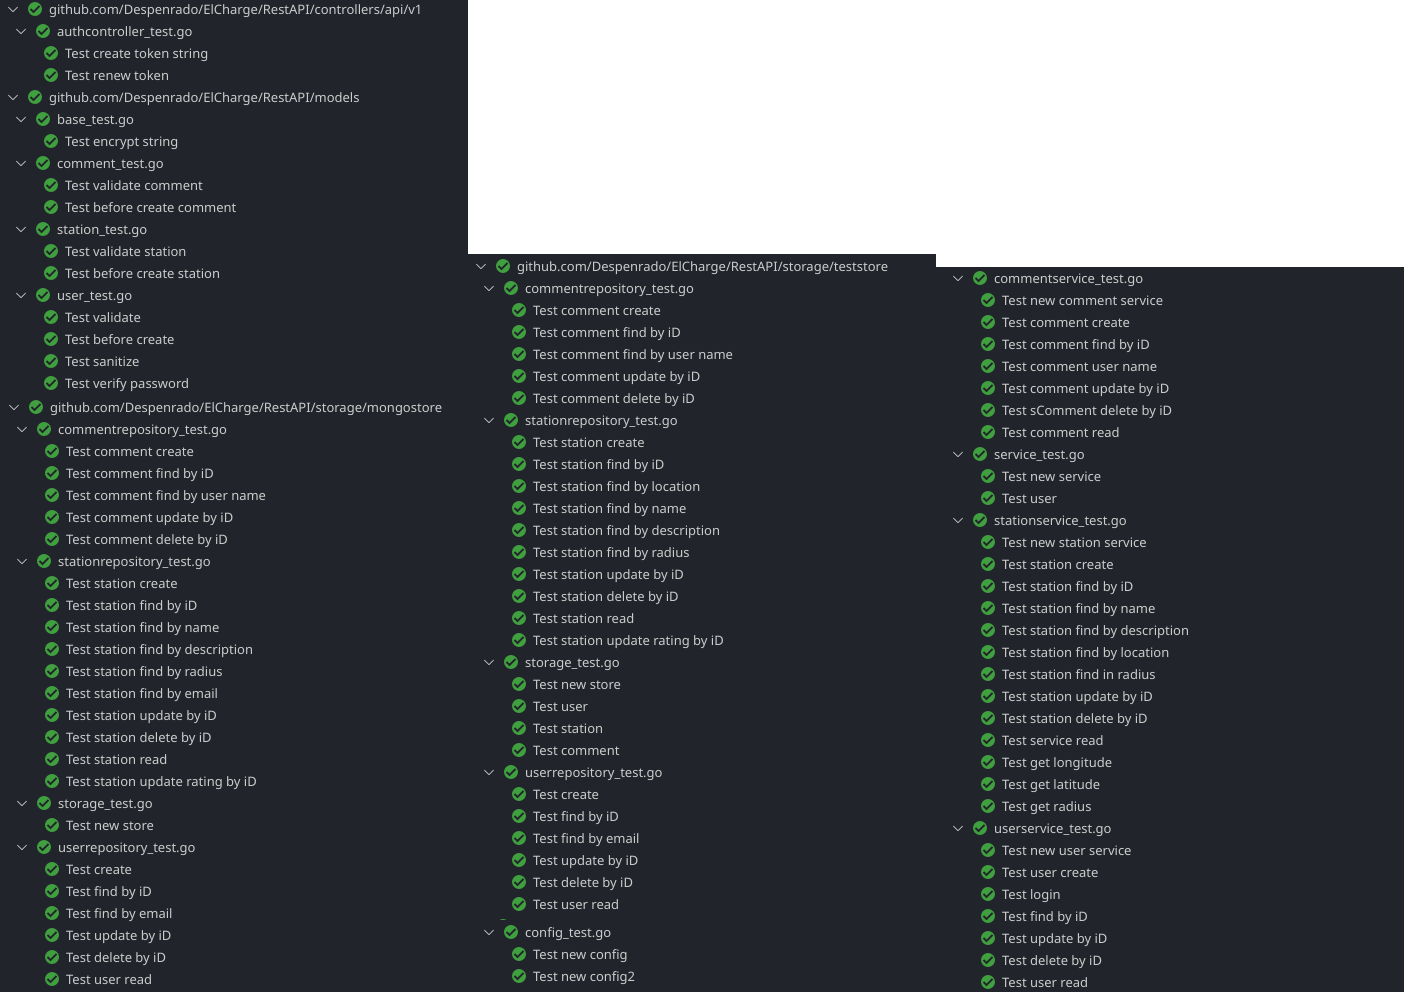
\includegraphics[width=1\linewidth]{rys04/test_list.png}
        \caption{Lista testów jednostkowych}
    \label{fig:test_list}
\end{figure}

% 
\section{Testy API}
Do testowania interfejsu API wykorzystano narzędzie do automatycznego testowania Postman.
Przeprowadzono testy wszystkich endpointów (rys. \ref{fig:postma_list}).
\begin{figure}[ht]
    \centering
        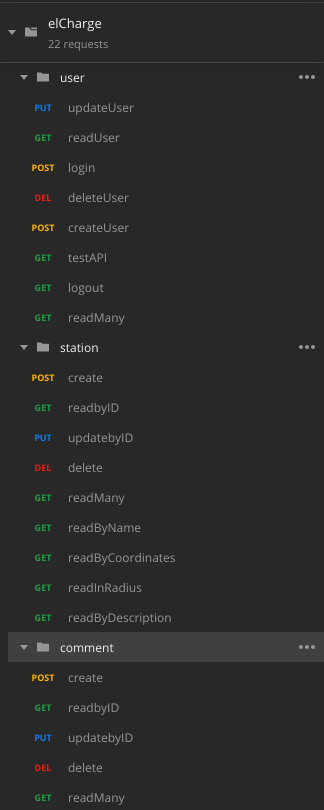
\includegraphics[width=0.3\linewidth]{rys04/postman_list.png}
        \caption{Lista testów API}
    \label{fig:postma_list}
\end{figure}
\newpage

Przykład testowania logowania (rys. \ref{fig:postman_login1}):
\begin{figure}[ht]
    \centering
        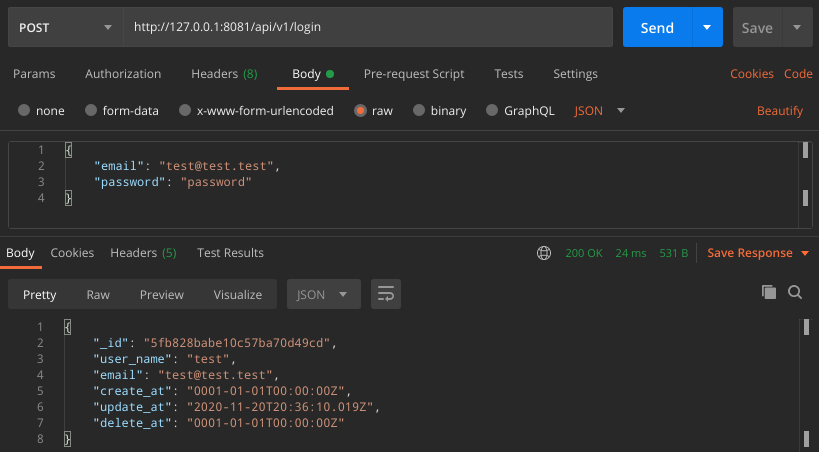
\includegraphics[width=0.9\linewidth]{rys04/postman_login1.png}
        \caption{Testowanie logowania za pomocą Postman}
    \label{fig:postman_login1}
\end{figure}

% TO DO: proszę zrzuty z Postmana robić przy zawężonym oknie (okienko nie może rozpinać się na całą szerokość ekranu, bo potem jak się wklei obrazek do dokumentu wychodzą za małe literki).
% TO VERIFY: Przerobiłem te obrazki, ale to nie do kończ rzuty, to sklejone rzuty, bo nie chciałem żeby zajmowało za dużo niejsca. Czy mam to jakoś zaznaczyć?
% TO DO: Proszę najpierw zawęzić okienko postmana, a potem wykonać zrzut (aplikacje okienkowe pozwalają na zmianę rozmiaru okna). Jak zmieni Pan rozmiar okna, wtedy elementy poukładają się bliżej siebie. Ostatecznie można przerobić obrazki w paincie
Przykład testowania tworzenia stacji ładującej samochody elektryczne (rys. \ref{fig:postman_create_station}).
\begin{figure}[ht]
    \centering
        \includegraphics[width=0.9\linewidth]{rys04/postman_create_station.png}
        \caption{Testowanie tworzenia stacji ładowanicej za pomocą Postman}
    \label{fig:postman_create_station}
\end{figure}

% Пример создания еомментария и его модификции.
Przykład tworzenia komentarza (rys. \ref{fig:postman_create_comment}) i jego modyfikacji (rys. \ref{fig:postman_edit_comment}).
\begin{figure}[ht]
    \centering
        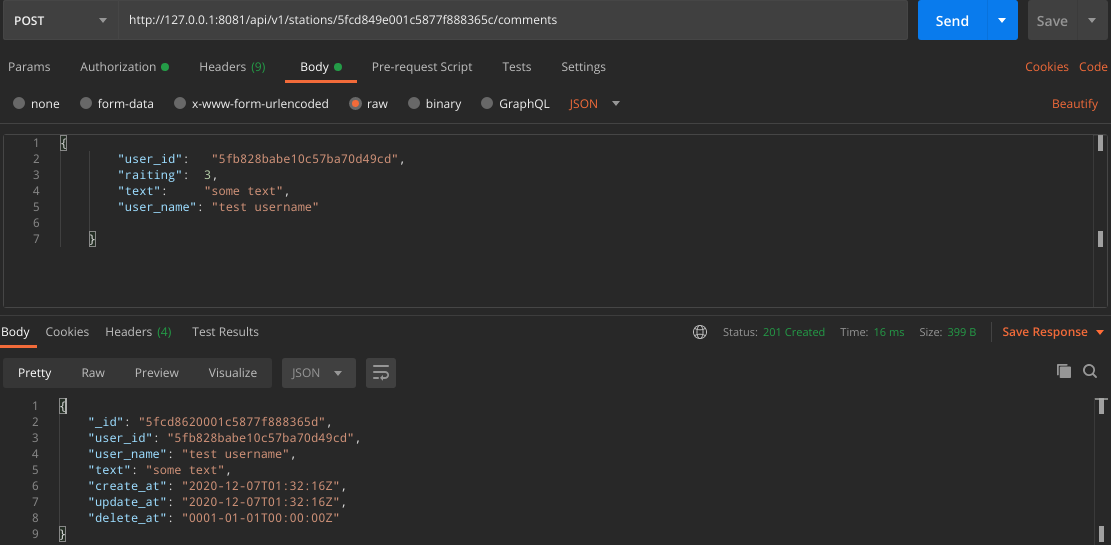
\includegraphics[width=0.9\linewidth]{rys04/postman_create_comment.png}
        \caption{Testowanie tworzenia komentarza za pomocą Postman}
    \label{fig:postman_create_comment}
\end{figure}
\begin{figure}[ht]
    \centering
        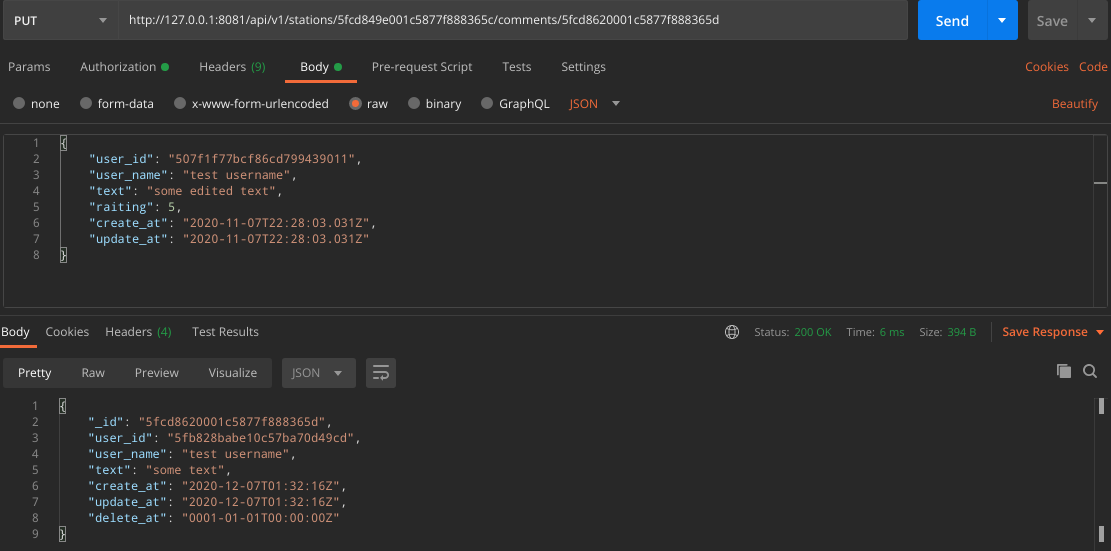
\includegraphics[width=0.9\linewidth]{rys04/postman_edit_comment.png}
        \caption{Testowanie edycji komentarza za pomocą Postman}
    \label{fig:postman_edit_comment}
\end{figure}
\newpage
% пример поиска зарядной станции в радиусе 100 км от установлиенных координат, а также лиммитирования списка:
Przykład wyszukiwania stacji ładującej (rys. \ref{fig:postman_find_stations}) w dystansie 100 km od ustalonych współrzędnych, a także ograniczenia listy:
\begin{figure}[ht]
    \centering
        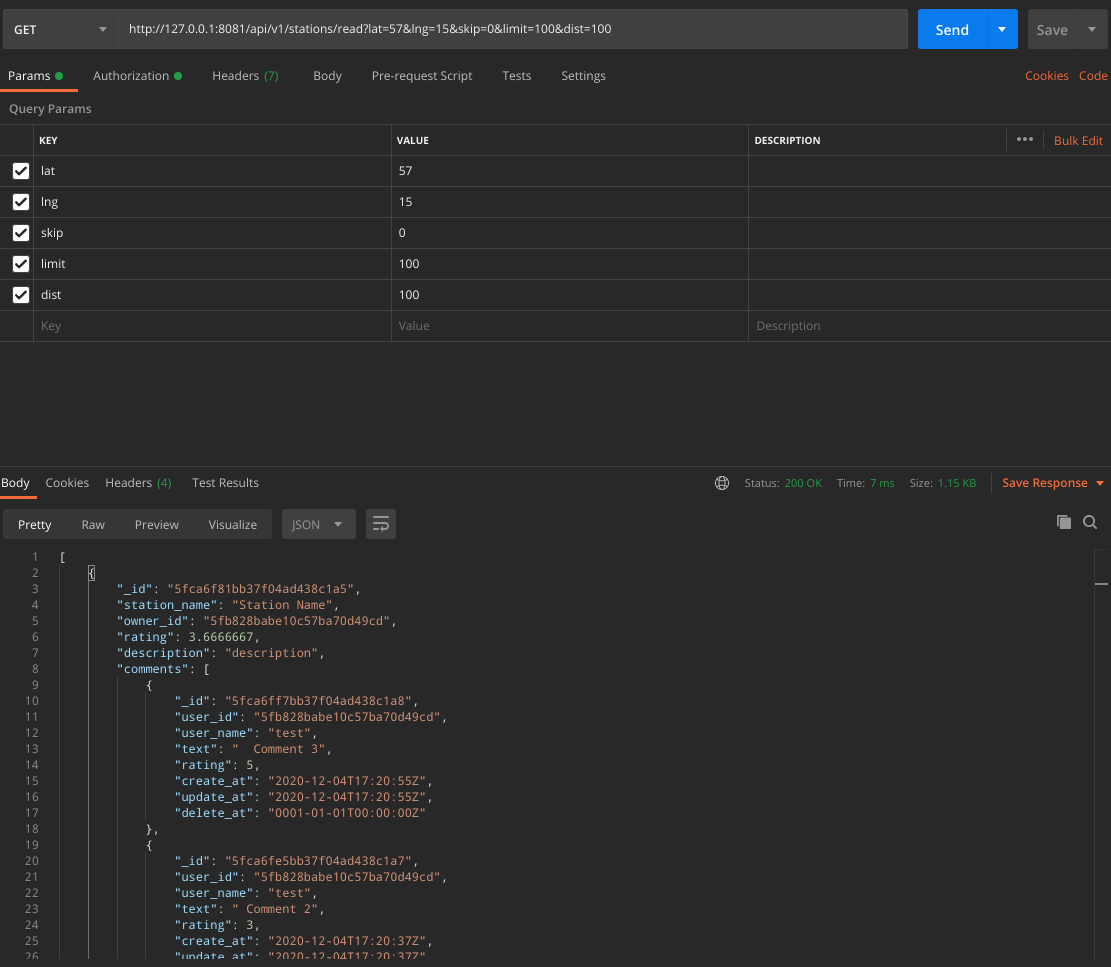
\includegraphics[width=0.9\linewidth]{rys04/postman_find_stations.png}
        \caption{Testowanie złożonego wyszukiwania stacji ładowniczej za pomocą Postman}
    \label{fig:postman_find_stations}
\end{figure}